\subsection{Spektrálna analýza}

Snáď najdôležitejšou aplikáciou fourierovej transformácie vo fyzike a
chémii je spektrálna interferometria. V tejto kapitole v skratke
rozvedieme najdôležitejšie pojmy a mechanizmy o tejto pre chemikov
životne dôležitej metóde skúmania látok.

Ako už názov naznačuje, spektrálna analýza má za úlohu analyzovať
látky. Deje sa tak prostredníctvom infračervených vĺn. Čitateľ by sa
mohol opýtať, prečo sa používajú tieto vlny a jeho zvedavosti bude za
chvíľu zadosťučinené.

\subsubsection{Chemické väzby}
Základom každej chemickej zlúčeniny sú atómy, medzi ktorými vznikajú
väzby. Väzba je akási neviditeľná pružina, ktorá vzniká ako dôsledok
pôsobenia elektromagenetickej a slabej jadrovej sily. Existuje istá
vzialenosť molekúl, keď sú tieto sily v rovnováhe a celková energia
väzby je minimálna. Vychýlením atómu zo svojej polohy prevládne jedna
z týchto dvoch síl a atóm má snahu dostať sa do svojej pôvodnej
polohy. Samozrejme, atómy za predpokladu bežnej teploty nestoja na
mieste ale kmitajú okolo rovnovážnej polohy a väzby ich držia pokope.

To čo je ale pri spektrálnej analýze dôležité je, že rôzne väzby sa
správajú rôzne. Kratšie väzby kmitajú rýchlejšie, väzba od ťažkých
atómov kmitá pomalšie, a takisto vlastnosti väzby závisia aj od
elektrických vlastností atómov. Preto sa každá väzba dá identifikovať
podľa svojej frekvencie kmitania. Prehľad niektorých vybraných typov
väzieb sa dá nájsť v tabuľke \ref{tab:vazby} (čiastočne prevzaná z \cite{wiki:spectro}).

\begin{table}[htb]
\centering
\begin{tabular}{| l | r | r |}
\hline
väzba & špecifický typ väzby & frekvencia ($\cm^{-1}$). \\ \hline
C-O & alkoholy & 1040-1060, 1100 \\ \hline
C-H & C=CH & 3020 \\ \hline
C-H & metyl & 1260 \\ \hline
C=O & aldehyd & 1725 \\ \hline
C-C & aromatické C=C & 1450, 1500, 1580, 1600 \\ \hline
O-H & alkoholy & 3200-3400 \\ \hline
N-H & amíny & 3400-3500, 1560-1640 \\ \hline
\end{tabular}
\caption{Ukážka absorbčných frekvencií väzieb}\label{tab:vazby}
\end{table}

Otázkou ale ostáva, ako odhaliť frekvenciu kmitania väzieb. Odpoveď
nám núka fyzika sama. Atómy sa bežne nachádzajú v základnom stave.
Avšak pôsobením žiarenia s frekvenciou rovnou frekvencii kmitania
väzby môžeme atóm rozkmitať ešte viac. Je to jav podobný rezonancii - 
vonkajším pôsobením vynútime kmity rezonátora - väzby.
Takto rozkmitaný atóm sa môže dostať do excitovaného stavu. Pri tomto
prechode medzi stavmi atóm pohltí energiu. Zo zákona zachovania
energie musí tým pádom dopadajúce žiarenie stratiť nejakú časť
energie. No a táto strata energie (na príslušnej frekvencii) je
základom pre spektrometriu.


\begin{poznamka}
Viac o chemických väzbách sa dá nájsť v \cite{wiki:bonds} a
\cite{Chem}. Taktiež na stránke \cite{webspectra} sa dá nájsť
interaktívny program na porovnávanie spektier.
\end{poznamka}

\subsubsection{Konštrukcia spektrometra}
Spektrometer môžeme rozdeliť na niekoľko základných častí.
\begin{itemize}
\item zdroj IR žiarenia 
\item Michaelsonov interferometer - zložený z takzvaného
``beamsplittera'' čo je polopriepustné zrkadlo, jedného fixného
a jedn=eho pohyblivého zrkadla
\item kryštál
\item detektor
\end{itemize}
Zjednodušenú schému spektrometra možno vidieť na obrázku
\ref{fig:ftir_schema}

\begin{figure}[htp]
\centering
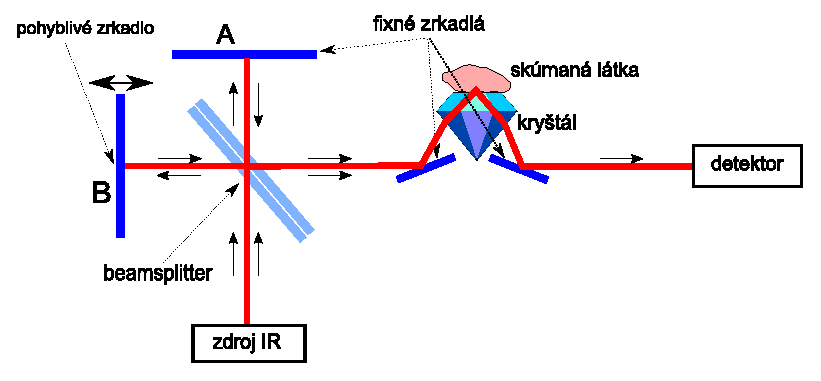
\includegraphics{obrazky/ftir_schema}
\caption{Základná konštrukcia spektrometra}\label{fig:ftir_schema}
\end{figure}

Infračervený lúč začne svoju púť v zdroji žiarenia. Obvylke je to 
cievka, ktorá je napájaná jednosmerným napätím a zohrieva sa.
Potom, ako lúč opustí zdroj, narazí na beamsplitter. Beamsplitter
je IR priehľadný materiál, napríklad KBr. Beamsplitter pôsobí
na lúč ako polopriehľadné zrkadlo. Približne jednu polovicu žiarenia
prepustí smerom na zrkadlo A, druhú polovicu smerom na zrkadlo B.
Žiarenia odrazené od zrkadla A sa opäť dostáva do beamsplittera,
časť pokračuje smerok ku kryštálu a časť sa vracia do zdroja.
Žiarenie odrazené od zrkadla B sa taktiež dostáva do beamsplittera a
opäť jedna časť sa vráti do zdroja a druhá časť pokračuje v smere na
kryštál. Nás bude odteraz zaujímať iba žiarenie smerujúce do kryštálu.
Toto žiarenie je zložením dvoch lúčov z toho istého zdroja, avšak
(vďaka tomu, že zrkadlo B je pohyblivé) tieto lúče majú istý
\todo{path difference}. Tieto lúče preto spolu interferujú a môžeme
uvažovať, ze ďalej pokračuje len jeden výsledný lúč.
Tento je pomocou zrkadiel nasmerovaný do kryštálu. Kryštál má zaistiť,
aby lúč


\subsubsection{Výpočet absorpcie}
Základom pre chemickú analýzu je graf $A(f)$ absorbcie materiálu v
závislosti od frekvencie. Absorbcia $A$ je definovaná ako
$A=-\log_{10} T$, kde $T$ je transmitancia. Transmitancia vlastne
znamená, akú veľkú časť žiarenia na danej frekvencii látka prepustí
a môžeme ju teda vyjadriť ako $T=I/I_0$ kde $I$ je intenzita
prepusteného žiarenia a $I_0$ je intenzita žiarenia dopadajúceho na
materiál.
Celkovo môžeme teda písať, že $A(f) = -\log_{10} \frac{I(f)}{I_0(f)}$.
Problém ale ostáva v určovaní $I(f), I_0(f)$. Detektor totiž nevie rozlíšiť
žiarenia jednotlivých frekvencií ale mieša ich všetky dokopy.
Výsledkom je jediná hodnota $i=\int_0^\infty I(f) df$
\footnote{Presnejšie povedané výsledkom nie je intenzita ale energia.
Za našich podmienok sú ale tieto 2 veličny priamo úmerné}.
Aby sme mohli z $I$ určiť $I(f)$, musíme použiť nasledujúci trik.

Nech $I(x)$ je hodnota nameraná detektorom, ak je zrkadlo B vo
vzdialenosti $x$ od beamsplittera. Pre našu pohodlnosť si ešte zavedieme,
že $x$ sa meria smerom zľava doprava. Ďalej nech $y$ je vzdialenosť zrkadla
A od beamsplittera a nech $I_z(f)$ je intenzita žiarenia o frekvencii
$f$ zdroja. Predpokladajme, že beamsplitter rozdelí žiarenia na 2 lúče
o rovnakej intenzite. Ak označíme $I_i$ intenzitu výstupného
žiarenia z beamsplittera po interferencii, môžeme písať
$I_i(f,x)=\frac{1}{4} I_z(f) p(f,x)$ kde $p$ je parameter ako sa budú
interferujúce lúče ovplyvňovať, $p \in <0,2>$. 
Konštantu $\frac{1}{4}$ sme získali ako dôsledok toho, že beamsplitter
každým prechodom lúč rozbije na 2 časti.
Parameter $p$ sme si zrátali v \todo{}, keď sme sa
bavili o interferencii svetelných lúčov. Pre poriadok ho uveďme ešte
raz
\begin{equation}
p(f,x)=A(f) \cos(\frac{\pi x}{\lambda}) + B(f)
\end{equation}
$\lambda=\frac{c}{f}$

Teda $I_i(f,x)= I_z(f) (A(f) \cos \frac{\pi x f}{c} + B(f))$. Potom
detektor zachytí intenzitu 
$I(x)=\int_0^\infty I_i(f,x) T(f)\,df$.
$I(x)=A(f) \int_0^\infty I_z(f) T(f) \cos \frac{\pi x f}{c}
df +\int_0^\infty B(f) I_z(f) T(f)\,df$.
$I(x)=A(f) \int_0^\infty (I_z(f) T(f)) \cos \frac{\pi x f}{c}\,df +
C$.

\todo{Zvysok}


